\chapter{Encoder Circuits}\label{ch09}

\begin{tcolorbox}[colback=blue!5!white,colframe=blue!75!black]
	% Upper half of box: my "title" area
	\textcolor{blue}{\textbf{What to Expect}}
	% Lower half of the box: the content
	\tcblower
	Encoders and decoders are used to change a coded byte from one form to another. For example, a binary-to-BCD encoder changes a binary byte to its \gls{bcd} equivalent. Encoders and decoders are very common in digital circuits and are used, for example, to change a binary number to a visual display that uses an \gls{led}. The following topics are included in this chapter.
	
	\begin{itemize}
		\item Developing circuits the use multiplexers and demultiplexers
		\item Creating a minterm generator using a multiplexers
		\item Creating a ten-line priority encoder
		\item Using a seven-segment display for a decoded binary number
		\item Employing a decoder as a function generator
		\item Explaining the theory and process of error detection and correction
		\item Detecting errors in a transmitted byte using the Hamming Code
	\end{itemize}
	
\end{tcolorbox}

\section{Multiplexers/Demultiplexers}
\label{CL:sec:multiplexers_demultiplexers}

\subsection{Multiplexer}
\label{CL:subsec:multiplexer}

\marginpar{A multiplexer is usually called a ``mux'' and a demultiplexer is called a ``dmux.''}

A multiplexer is used to connect one of several input lines to a single output line. Thus, it selects which input to pass to the output. This function is similar to a rotary switch where several potential inputs to the switch can be sent to a single output. A demultiplexer is a multiplexer in reverse, so a single input can be routed to any of several outputs. While mux/dmux circuits were originally built for transmission systems (like using a single copper wire to carry several different telephone calls simultaneously), today they are used as ``decision-makers'' in virtually every digital logic system and are, therefore, one of the most important devices for circuit designers. 

To help clarify this concept, Figure \ref{CL:fig:multiplexer_using_rotary_switches} is a simple schematic diagram that shows two rotary switches set up as a mux/dmux pair. As the switches are set in the diagram, a signal would travel from \textsf{INPUT B} to \textsf{OUTPUT 2} through a connecting wire. 

\begin{figure}[H]
  \caption{Multiplexer Using Rotary Switches}
  \label{CL:fig:multiplexer_using_rotary_switches}  
  \myfloatalign
  \begin{tikzpicture} [circuit logic US, scale=1.00]
  % make all path lines (the node shapes) a little thicker
  \tikzstyle{every path}=[line width=0.50mm]  
  
  % Input nodes
  \node[circ,label={135:A}] (nA) at (0.40,2.50) {};
  \node[circ,label={180:B}] (nB) at (0.15,2.35) {};
  \node[circ,label={180:C}] (nC) at (0.0,2.00) {};
  \node[circ,label={180:D}] (nD) at (0.15,1.65) {};
  \node[circ,label={225:E}] (nE) at (0.40,1.50) {};
  % Connector Nodes
  \node[circ] (c01) at (0.5,2.00) {};
  \node[circ] (c02) at (2.0,2.00) {};  
  % Output nodes
  \node[circ,label={45:1}] (o1)  at (2.1,2.50) {};
  \node[circ,label={0:2}]  (o2)  at (2.35,2.35) {};
  \node[circ,label={0:3}]  (o3)  at (2.5,2.00) {};
  \node[circ,label={0:4}]  (o4)  at (2.35,1.65) {};
  \node[circ,label={315:5}] (o5) at (2.1,1.50) {};
  
  % Draw the lines
  \pgfsetarrowsend{latex};
  \draw (c01) -- (nB);
  \draw (c02) -- (o2);

  \pgfsetarrowsend{};
  \draw (c02) -- (c01) ;    
  \end{tikzpicture}
\end{figure}

Imagine that the switches could somehow be synchronized so they rotated among the setting together; that is, \textsf{INPUT A}  would always connect to \textsf{OUTPUT 1} and so forth. That would mean a single wire could carry five different signals. For example, imagine that the inputs were connected to five different intrusion sensors in a building and the five outputs were connected to lamps on a guard's console in a remote building. If something triggered sensor $ A $ then as soon as the mux/dmux pair rotated to that position it would light lamp one on the console. Carrying all of these signals on a single wire saves a lot of expense. Of course, a true alarm system would be more complex than this, but this example is only designed to illustrate how a mux/dmux pair works in a transmission system.

Figure \ref{fig:08_01} is the logic diagram for a simple one-bit two-to-one multiplexer. In this circuit, an input is applied to input ports \emph{A} and \emph{B}. Port \emph{Sel} is the selector and if that signal is zero then Port \emph{A} will be routed to output \emph{Y}; if, though, \emph{Sel} is one then Port \emph{B} will be routed to \emph{Y}.

\begin{figure}[H]
	\centering
	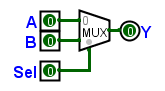
\includegraphics[width=\maxwidth{.95\linewidth}]{gfx/08_01}
	\caption{Simple Mux}
	\label{fig:08_01}
\end{figure}

Truth Table \ref{tab:08_01}, below, is for a multiplexer:

\begin{table}[H]
  \sffamily
  \newcommand{\head}[1]{\textcolor{white}{\textbf{#1}}}    
  \begin{center}
    \rowcolors{2}{gray!10}{white} % Color every other line a light gray
    \begin{tabular}{cc|cc} 
      \rowcolor{black!75}
      \multicolumn{3}{c}{\head{Inputs}} & \head{Output} \\
      A & B & Sel & Y \\
      \hline
      0 & 0 & 0 & 0 \\
      0 & 0 & 1 & 0 \\
      0 & 1 & 0 & 0 \\
      0 & 1 & 1 & 1 \\
      1 & 0 & 0 & 1 \\
      1 & 0 & 1 & 0 \\
      1 & 1 & 0 & 1 \\
      1 & 1 & 1 & 1 
    \end{tabular}
  \end{center}
  \caption{Truth Table for a Multiplexer}
  \label{tab:08_01}
\end{table}

In this multiplexer, the data input ports are only a single bit wide; however, in a normal circuit those ports could be a full $ 32 $-bit or $ 64 $-bit word and the selected word would be passed to the output port. Moreover, a multiplexer can have more than two input ports so a very versatile switch can be built to handle switching full words from one of eight or even sixteen different inputs. Because of its ability to channel a selected data stream to a single bus line from many different sub-circuits, the multiplexer is one of the workhorses for digital logic circuits and is frequently found in complex devices like \glspl{cpu}.
 
\subsection{Demultiplexer}
\label{CL:subsec:demultiplexer}

A demultiplexer is the functional opposite of a multiplexer: a single input is routed to one of several potential outputs. Figure \ref{fig:08_02} is the logic diagram for a one-bit one-to-two demultiplexer. In this circuit, an input is applied to input port \emph{A}. Port \emph{Sel} is a control signal and if that signal is zero then input \emph{A} will be routed to output \emph{Y}, but if the control signal is one then input \emph{A} will be routed to output \emph{Z}.

\begin{figure}[H]
	\centering
	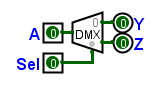
\includegraphics[width=\maxwidth{.95\linewidth}]{gfx/08_02}
	\caption{Simple Dmux}
	\label{fig:08_02}
\end{figure}

Truth Table \ref{tab:08_02}, below, is for a demultiplexer.

\begin{table}[H]
  \sffamily
  \newcommand{\head}[1]{\textcolor{white}{\textbf{#1}}}    
  \begin{center}
    \rowcolors{2}{gray!10}{white} % Color every other line a light gray
    \begin{tabular}{cc|cc} 
      \rowcolor{black!75}
      \multicolumn{2}{c}{\head{Inputs}} & \multicolumn{2}{c}{\head{Outputs}} \\
      A & Sel & Y & Z \\
      \hline
      0 & 0 & 0 & 0 \\
      0 & 1 & 0 & 0 \\
      1 & 0 & 0 & 1 \\
      1 & 1 & 1 & 0 
    \end{tabular}
  \end{center}
  \caption{Truth Table for a Demultiplexer}
  \label{tab:08_02}
\end{table}

In this demultiplexer the data input port is only a single bit wide; however, in a normal circuit that port could be a full $ 32 $-bit or $ 64 $-bit word and that entire word would be passed to the selected output port. Moreover, a demultiplexer can have more than two outputs so a very versatile switch can be built to handle switching full words to one of eight or even sixteen different outputs. Because of its ability to switch a data stream to different sub-circuits, the demultiplexer is one of the workhorses for digital logic circuits and is frequently found in complex devices like \glspl{cpu}.

\subsection{Minterm Generators}
\label{CL:subsec:minterm_generators}

Demultiplexers can be combined with an \textsf{OR} gate and be used as a minterm generator. Consider the circuit for this two-variable equation.

\begin{align}
  \label{CL:eq:2_var_minterm_gen}
  \int(A,B) &= \sum(1,2)
\end{align}

Since there are two input variables, \emph{A} and \emph{B}, the dmux needs to have two select bits, one for each variable, and that would generate four potential dmux outputs \emph{W}, \emph{X}, \emph{Y}, and \emph{Z}. This circuit could be constructed using a four-output dmux with a two-bit control signal.

\begin{figure}[H]
	\centering
	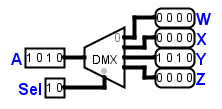
\includegraphics[width=\maxwidth{.95\linewidth}]{gfx/08_03}
	\caption{1-to-4 Dmux}
	\label{fig:08_03}
\end{figure}

In Figure \ref{fig:08_03}, a four-bit input (\emph{A}) is routed to one of four output ports: \emph{W}, \emph{X}, \emph{Y}, or \emph{Z}, depending on the setting of the select, \emph{Sel}. Figure \ref{fig:08_03} shows the data input of $ 1010 $ being routed to \emph{Y} by a select of $ 10 $.

However, the equation specifies that the only outputs that would be used are when \emph{Sel} is $ 01 $ or $ 10 $. Thus, output ports \emph{X} and \emph{Y} must be sent to an \textsf{OR} gate and the other two outputs ignored. The output of the \textsf{OR} gate would only activate when \emph{Sel} is set to $ 01 $ or $ 10 $, as shown in Figure \ref{fig:08_04}. 

\begin{figure}[H]
	\centering
	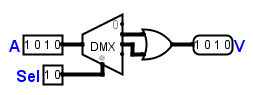
\includegraphics[width=\maxwidth{.95\linewidth}]{gfx/08_04}
	\caption{1-to-4 Dmux As Minterm Generator}
	\label{fig:08_04}
\end{figure}


\section{Encoders/Decoders}
\label{CL:sec:encoders_decoders}

\subsection{Introduction}
\label{CL:subsec:introduction_to_encoders_decoders}

Encoders and decoders are used to convert some sort of coded data into a different code. For example, it may be necessary to convert the code created by a keyboard into \gls{ascii} for use in a word processor. By definition, the difference between an encoder and a decoder is the number of inputs and outputs: Encoders have more inputs than outputs, while decoders have more outputs than inputs. 

As an introduction to encoders, consider Figure \ref{fig:08_14}, which is designed to encode three single line inputs (maybe three different push buttons on a control panel) into a binary number for further processing by the computer. In this circuit, the junction between the two \textsf{OR} gates and the output ($ Y $) is a \emph{joiner} that combines two bit streams into a single bus. Physically, two wires (one from \emph{U1} and one from \emph{U2}) would be spliced together into a single cable (a \emph{bus}) that contains two strands. The figure shows that when input \emph{C} is active the output of the encoder is $ 11 $.

\begin{figure}[H]
	\centering
	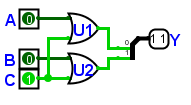
\includegraphics[width=\maxwidth{.95\linewidth}]{gfx/08_14}
	\caption{Three-line to 2-Bit Encoder}
	\label{fig:08_14}
\end{figure}
 
As an introduction to decoders, consider Figure \ref{fig:08_15}, which is designed to decode a two-bit binary input and drive a single output line high. A circuit like this may be used to light an \gls{led} used as a warning on a console if a particular binary code is generated elsewhere in a circuit. In this circuit, the input is a two-bit number ($ 10 $ in the illustration), but those two bits are separated through a splitter and each is applied to one of the inputs of a series of four \textsf{AND} gates. Imagine that the \gls{msb} was placed on the wire on the left of the grid and wired to the bottom input of each of the \textsf{AND} gates. If $ A=10 $, then \textsf{AND} gate three would activate and output \emph{X} would go high.

\begin{figure}[H]
	\centering
	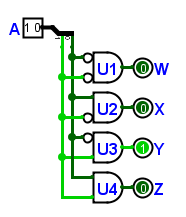
\includegraphics[width=\maxwidth{.95\linewidth}]{gfx/08_15}
	\caption{Four-Bit to 4-Line Decoder}
	\label{fig:08_15}
\end{figure}

Both encoders and decoders are quite common and are used in many electronic devices. However, it is not very common to build these circuits out of discrete components (like in the circuits above). Rather, inexpensive integrated circuits are available for most encoder/decoder operations and these are much easier, and more reliable, to use. 

\subsection{Ten-Line Priority}
\label{CL:subsec:10_line_priority}

\marginpar{This encoder is sometimes called Ten-Line to Four-Line.}

Consider a ten-key keypad containing the numbers zero through nine, like a keypad that could be used for numeric input from some hand-held device. In order to be useful, a key press would need to be encoded to a binary number for further processing by a logic circuit. 

The keypad outputs a nine-bit number such that a single bit goes high to indicate which key was. For example, when key number two is pressed, $ 0\_0000\_0010 $ is output from the device. A priority encoder would accept that nine-bit number and output a binary number that could be used in computer circuits. Truth Table \ref{CL:tab:truth_table_for_priority_encoder} is for the Priority Encoder that meets the specification. The device is called a ``priority'' encoder since it will respond to only the highest value key press. For example, if someone pressed the three and five keys simultaneously the encoder would ignore the three key press and transmit $ 0101 $, or binary five.\marginpar{Dashes are normally used to indicate ``don't care'' on a Truth Table.}

\begin{table}[H]
  \sffamily
  \newcommand{\head}[1]{\textcolor{white}{\textbf{#1}}}    
  \begin{center}
    \rowcolors{2}{gray!10}{white} % Color every other line a light gray
    \begin{tabular}{ccccccccc|cccc} 
      \rowcolor{black!75}
      \multicolumn{9}{c}{\head{Inputs}} & \multicolumn{4}{c}{\head{Outputs}} \\
      9 & 8 & 7 & 6 & 5 & 4 & 3 & 2 & 1 & Y1 & Y2 & Y3 & Y4 \\
      \hline
      0 & 0 & 0 & 0 & 0 & 0 & 0 & 0 & 1 & 0 & 0 & 0 & 1 \\
      0 & 0 & 0 & 0 & 0 & 0 & 0 & 1 & - & 0 & 0 & 1 & 0 \\
      0 & 0 & 0 & 0 & 0 & 0 & 1 & - & - & 0 & 0 & 1 & 1 \\
      0 & 0 & 0 & 0 & 0 & 1 & - & - & - & 0 & 1 & 0 & 0 \\
      0 & 0 & 0 & 0 & 1 & - & - & - & - & 0 & 1 & 0 & 1 \\
      0 & 0 & 0 & 1 & - & - & - & - & - & 0 & 1 & 1 & 0 \\
      0 & 0 & 1 & - & - & - & - & - & - & 0 & 1 & 1 & 1 \\
      0 & 1 & - & - & - & - & - & - & - & 1 & 0 & 0 & 0 \\
      1 & - & - & - & - & - & - & - & - & 1 & 0 & 0 & 1
    \end{tabular}
  \end{center}
  \caption{Truth Table for Priority Encoder}
  \label{CL:tab:truth_table_for_priority_encoder}
\end{table}

This circuit can be realized by using a grid input and routing the various lines to an appropriate \emph{AND} gate. This is one of the circuits built in the lab manual that accompanies this text.

\subsection{Seven-Segment Display}
\label{CL:subsec:7_segment_display}

A seven-segment display is commonly used in calculators and other devices to show hexadecimal numbers. To create the numeric shapes, various segments are activated while others remain off, so binary numbers must be decoded to turn on the various segments for any given combination of inputs. A seven-segment display has eight input ports and, when high, each of those ports will activate one segment of the display. 

\begin{figure}[H]
  \caption{Seven-Segment Display}
  \label{CL:fig:seven_segment_display}  
  \myfloatalign
  \begin{tikzpicture} [circuit logic US, scale=1.00]
    \SSGLeg[3em]{};
    \SSGNb[3em]{}{2};
  \end{tikzpicture}
\end{figure}
 
\marginpar{Usually an eighth ``segment'' is available \textemdash a decimal point in the lower right corner.}

In Figure \ref{CL:fig:seven_segment_display} the seven segments are labeled and it shows that the number ``$ 2 $'' for example, is made by activating segments \textsf{a}, \textsf{b}, \textsf{g}, \textsf{e}, and \textsf{d}. Table \ref{CL:tab:truth_table_for_seven_segment_display} shows the various segments that must be activated for each of the $ 16 $ possible input values.

\begin{table}[H]
  \sffamily
  \newcommand{\head}[1]{\textcolor{white}{\textbf{#1}}}    
  \begin{center}
    \rowcolors{2}{gray!10}{white} % Color every other line a light gray
    \begin{tabular}{cccccccccccccc} 
      \rowcolor{black!75}
      \head{Hex} & \head{|} & \multicolumn{4}{c}{\head{Binary}} & \head{|} & \multicolumn{7}{c}{\head{Display}} \\
        &|& \textbf{3} & \textbf{2} & \textbf{1} & \textbf{0} &|& \textbf{a} & \textbf{b} & \textbf{c} & \textbf{d} & \textbf{e} & \textbf{f} & \textbf{g} \\
%      0 &|& 0 & 0 & 0 & 0 &|& a & b & c & d & e & f & g \\
      0 &|& 0 & 0 & 0 & 0 &|& 1 & 1 & 1 & 1 & 1 & 1 & 0 \\
      1 &|& 0 & 0 & 0 & 1 &|& 0 & 1 & 1 & 0 & 0 & 0 & 0 \\
      \textbf{2} &|& \textbf{0} & \textbf{0} & \textbf{1} & 
        \textbf{0} &|& \textbf{1} & \textbf{1} & \textbf{0} & 
        \textbf{1} & \textbf{1} & \textbf{0} & \textbf{1} \\
      3 &|& 0 & 0 & 1 & 1 &|& 1 & 1 & 1 & 1 & 0 & 0 & 1 \\
      4 &|& 0 & 1 & 0 & 0 &|& 0 & 1 & 1 & 0 & 0 & 1 & 1 \\
      5 &|& 0 & 1 & 0 & 1 &|& 1 & 0 & 1 & 1 & 0 & 1 & 1 \\
      6 &|& 0 & 1 & 1 & 0 &|& 1 & 0 & 1 & 1 & 1 & 1 & 1 \\
      7 &|& 0 & 1 & 1 & 1 &|& 1 & 1 & 1 & 0 & 0 & 0 & 0 \\
      8 &|& 1 & 0 & 0 & 0 &|& 1 & 1 & 1 & 1 & 1 & 1 & 1 \\
      9 &|& 1 & 0 & 0 & 1 &|& 1 & 1 & 1 & 1 & 0 & 1 & 1 \\
      A &|& 1 & 0 & 1 & 0 &|& 1 & 1 & 1 & 0 & 1 & 1 & 1 \\
      B &|& 1 & 0 & 1 & 1 &|& 0 & 0 & 1 & 1 & 1 & 1 & 1 \\
      C &|& 1 & 1 & 0 & 0 &|& 1 & 0 & 0 & 1 & 1 & 1 & 0 \\
      D &|& 1 & 1 & 0 & 1 &|& 0 & 1 & 1 & 1 & 1 & 0 & 1 \\
      E &|& 1 & 1 & 1 & 0 &|& 1 & 0 & 0 & 1 & 1 & 1 & 1 \\
      F &|& 1 & 1 & 1 & 1 &|& 1 & 0 & 0 & 0 & 1 & 1 & 1 
    \end{tabular}
  \end{center}
  \caption{Truth Table for Seven-Segment Display}
  \label{CL:tab:truth_table_for_seven_segment_display}
\end{table}

Notice that to display the number ``$ 2 $'' (in bold font), segments \textsf{a}, \textsf{b}, \textsf{d}, \textsf{e}, and \textsf{g} must be activated. 

A decoder circuit, as in Figure \ref{fig:08_16}, uses a demultiplexer to activate a one-bit line based on the value of the binary input. Note: to save space, two parallel decoders are used in this circuit.

\begin{figure}[H]
	\centering
	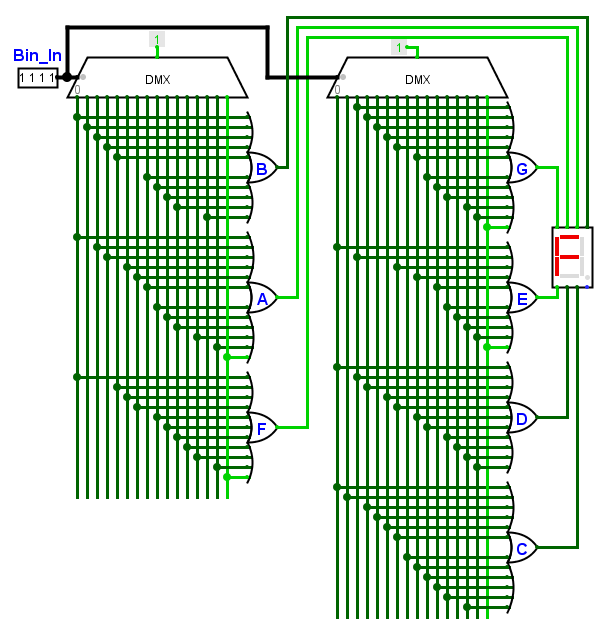
\includegraphics[width=\maxwidth{.95\linewidth}]{gfx/08_16}
	\caption{7-Segment Decoder}
	\label{fig:08_16}
\end{figure}

Figure \ref{fig:08_16} shows an input of $ 1111_2 $ so the last line on each demultiplexer is activated. Those lines are used to activate the necessary inputs on the seven-segment display to create an output of ``F''. 

A Hex Digit Display has a single port that accepts a four-bit binary number and that number is decoded into a digital display. Figure \ref{fig:08_17} shows a hex digit display. 

\begin{figure}[H]
	\centering
	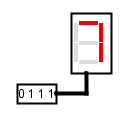
\includegraphics[width=\maxwidth{.95\linewidth}]{gfx/08_17}
	\caption{Hex Decoder}
	\label{fig:08_17}
\end{figure}

The \Le simulator used in this class includes both a \emph{7-Segment Display} and a \emph{Hex Digit Display}. One of the strengths of using a seven-segment display rather than a hex digit display is that the circuit designer has total control over which segments are displayed. It is common, for example, to activate each of the outer segments in a rapid sequence to give the illusion of a rotating circle. As opposed to a seven-segment display, a hex digit display is very simple to wire and use, as Figures \ref{fig:08_16} and \ref{fig:08_17} make clear. Both of these two types of displays are available on the market and a designer would chose whichever type meets the needs. 

\subsection{Function Generators}
\label{CL:subsec:function_generators}

Decoders provide an easy way to create a circuit when given a minterm function. Imagine that a circuit is needed for the function defined in Equation \ref{CL:eq:decoder_as_minterm_gen}.

\begin{align}
  \label{CL:eq:decoder_as_minterm_gen}
  \int(A,B,C) &= \sum(0,2,7)
\end{align}

Whatever this circuit is designed to do, it should activate an output only when the input is zero, two, or seven. The circuit in Figure \ref{fig:08_18} illustrates a simple minterm generator using a demultiplexer and an \textsf{OR} gate. When input \emph{A} is zero, two, or seven then output \emph{Y} will go high, otherwise it is low.

\begin{figure}[H]
	\centering
	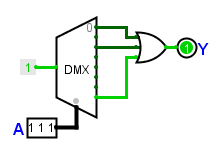
\includegraphics[width=\maxwidth{.95\linewidth}]{gfx/08_18}
	\caption{Minterm Generator}
	\label{fig:08_18}
\end{figure}

\section{Error Detection}
\label{CL:sec:error_detection}

\subsection{Introduction}
\label{CL:subsec:introduction_to_error_detection}

Whenever a byte (or any other group of bits) is transmitted or stored, there is always the possibility that one or more bits will be accidentally complemented. Consider these two binary numbers:

\begin{verbatim}
     0110 1010 0011 1010
     0110 1010 0111 1010
\end{verbatim} 

They differ by only one bit (notice Group Three). If the top number is what is supposed to be in a memory location but the bottom number is what is actually there then this would, obviously, create a problem. There could be any number of reasons why a bit would be wrong, but the most common is some sort of error that creeps in while the byte is being transmitted between two stores, like between a \gls{usb} drive and memory or between two computers sharing a network. It is desirable to be able to detect that a byte contains a bad bit and, ideally, even know which bit is wrong so it can be corrected. 

Parity is a common method used to check data for errors and it can be used to check data that has been transmitted, held in memory, or stored on a hard drive. The concept of parity is fairly simple: A bit (called the \emph{parity bit}) is added to each data byte and that extra bit is either set to zero or one in order to make the bit-count of that byte contain an even or odd number of ones. For example, consider this binary number: 

\begin{verbatim}
     1101
\end{verbatim}

There are three ones in this number, which is an odd number. If odd parity is being used in this circuit, then the parity bit would be zero so there would be an odd number of ones in the number. However, if the circuit is using even parity, then the parity bit would be set to one in order to have four ones in the number, which is an even number. Following is the above number with both even and odd parity bits (those parity bits are in the least significant position and are separated from the original number by a space for clarity): 

\begin{verbatim}
     1101 0 (Odd Parity)
     1101 1 (Even Parity)
\end{verbatim}

Table \ref{CL:tab:even_parity_examples} shows several examples that may help to clarify this concept. In each case, a parity bit is used to make the data byte even parity (spaces were left in the data byte for clarity). 

\begin{table}[H]
  \sffamily
  \newcommand{\head}[1]{\textcolor{white}{\textbf{#1}}}    
  \begin{center}
    \rowcolors{2}{gray!10}{white} % Color every other line a light gray
    \begin{tabular}{cc} 
      \rowcolor{black!75}
      \head{Data Byte} & \head{Parity Bit} \\
      0000 0000 & 0 \\
      0000 0001 & 1 \\
      0000 0011 & 0 \\
      0000 0100 & 1 \\
      1111 1110 & 1 \\
      1111 1111 & 0
    \end{tabular}
  \end{center}
  \caption{Even Parity Examples}
  \label{CL:tab:even_parity_examples}
\end{table}

Generating a parity bit can be done with a series of cascading \emph{XOR} gates but \Le had two parity gates, one that outputs high when the inputs have an odd number of ones and the other when there are an even number of ones. Figure \ref{fig:08_19} illustrates using an odd parity gate (labeled ``2K+1''). In this circuit, if input \emph{A} has an odd number of ones, as illustrated, then the parity generator will output a one to indicate input \emph{A} has an odd number of ones. That parity bit is added as the most significant bit to output \emph{Y}. Since output \emph{Y} will always have an even number of bits this is an even parity circuit.

\begin{figure}[H]
	\centering
	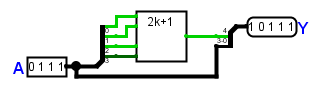
\includegraphics[width=\maxwidth{.95\linewidth}]{gfx/08_19}
	\caption{Parity Generator}
	\label{fig:08_19}
\end{figure}

Parity is a simple concept and is the foundation for one of the most basic methods of error checking. As an example, if some byte is transmitted using even parity but the data arrives with an odd number of ones then one of the bits was changed during transmission. 

\subsection{Iterative Parity Checking}
\label{CL:subsec:iterative_parity_checking}

One of the problems with using parity for error detection is that while it may be known that \emph{something} is wrong, there is no way to know which of the bits is wrong. For example, imagine an eight-bit system is using even parity and receives this data and parity bit:

\begin{verbatim}
     1001 1110 PARITY: 0
\end{verbatim} 

There is something wrong with the byte. It is indicating even parity but has an odd number of ones in the byte. It is impossible to know which bit changed during transmission. In fact, it may be that the byte is correct but the parity bit itself changed (a \emph{false error}). It would be nice if the parity error detector would not only indicate that there was an error, but could also determine which bit changed so it could be corrected. 

One method of error correction is what is known as \emph{Iterative Parity Checking}. Imagine that a series of eight-bit bytes were being transmitted. Each byte would have a parity bit attached; however, there would also be a parity byte that contains a parity bit for each bit in the preceding five bytes. It is easiest to understand this by using a table (even parity is being used):

\begin{table}[H]
  \sffamily
  \newcommand{\head}[1]{\textcolor{white}{\textbf{#1}}}    
  \begin{center}
    \rowcolors{2}{gray!10}{white} % Color every other line a light gray
    \begin{tabular}{cccccccccc} 
      \rowcolor{black!75}
      \head{Byte} & \multicolumn{8}{c}{\head{Data}} & \head{Parity} \\
      1 & 0 & 0 & 0 & 0 & 0 & 0 & 0 & 0 & 0 \\
      2 & 1 & 0 & 1 & 1 & 0 & 0 & 0 & 0 & 1 \\
      3 & 1 & 0 & 1 & 1 & 0 & 0 & 1 & 1 & 1 \\
      4 & 1 & 1 & 1 & 0 & 1 & 0 & 1 & 0 & 1 \\
      5 & 0 & 1 & 0 & 0 & 0 & 0 & 0 & 0 & 1 \\
      P & 1 & 0 & 1 & 0 & 1 & 0 & 0 & 1 & 0
    \end{tabular}
  \end{center}
  \caption{Iterative Parity}
  \label{CL:tab:iterative_parity}
\end{table}
 
In Table \ref{CL:tab:iterative_parity}, Byte one is $ 0000\;0000 $. Since the system is set for even parity, and it is assumed that a byte with all zeros is even, then the parity bit is zero. Each of the five bytes has a parity bit that is properly set such that each byte (with the parity bit) includes an even number of bits. Then, after a group of five bytes a \emph{parity byte} is inserted into the data stream so that each column of five bits also has a parity check; and that parity bit is found in row $ P $ on the table. Thus, the parity bit at the bottom of the first column is one since that column has three other ones. As a final check, the parity byte itself also has a parity bit added. 

Table \ref{CL:tab:iterative_parity_with_error} is the same as Table \ref{CL:tab:iterative_parity}, but Bit Zero, the least significant bit, in Byte One has been changed from a zero to a one (that number is highlighted).

\begin{table}[H]
  \sffamily
  \newcommand{\head}[1]{\textcolor{white}{\textbf{#1}}}    
  \begin{center}
    \rowcolors{2}{gray!10}{white} % Color every other line a light gray
    \begin{tabular}{cccccccccc} 
      \rowcolor{black!75}
      \head{Byte} & \multicolumn{8}{c}{\head{Data}} & \head{Parity} \\
      1 & 0 & 0 & 0 & 0 & 0 & 0 & 0 & \cellcolor{yellow!70!white}1 & 0 \\
      2 & 1 & 0 & 1 & 1 & 0 & 0 & 0 & 0 & 1 \\
      3 & 1 & 0 & 1 & 1 & 0 & 0 & 1 & 1 & 1 \\
      4 & 1 & 1 & 1 & 0 & 1 & 0 & 1 & 0 & 1 \\
      5 & 0 & 1 & 0 & 0 & 0 & 0 & 0 & 0 & 1 \\
      P & 1 & 0 & 1 & 0 & 1 & 0 & 0 & 1 & 0
    \end{tabular}
  \end{center}
  \caption{Iterative Parity With Error}
  \label{CL:tab:iterative_parity_with_error}
\end{table}

In Table \ref{CL:tab:iterative_parity_with_error} the parity for Byte One is wrong, and the parity for Bit Zero in the parity byte is wrong; therefore, Bit Zero in Byte One needs to be changed. If the parity bit for a row is wrong, but no column parity bits are wrong, or a column is wrong but no rows are wrong, then the parity bit itself is incorrect. This is one simple way to not only detect data errors, but correct those errors. 

There are two weaknesses with iterative parity checking. First, it is restricted to only single-bit errors. If more than one bit is changed in a group then the system fails. This, though, is a general weakness for most parity checking schemes. The second weakness is that a parity byte must be generated and transmitted for every few data bytes (five in the example). This increases the transmission time dramatically and normally makes the system unacceptably slow.

\subsection{Hamming Code}
\label{CL:subsec:hamming_code}

\subsubsection{Introduction}
\label{CL:subsubsec:introduction_to_hamming_code}

Richard Hamming worked at Bell labs in the $ 1940 $s and he devised a way to not only detect that a transmitted byte had changed, but exactly which bit had changed by interspersing parity bits within the data itself. Hamming first defined the ``distance'' between any two binary words as the number of bits that were different between them. As an example, the two binary numbers $ 1010 $ and $ 1010 $ has a distance of zero between them since there are no different bits, but $ 1010 $ and $ 1011 $ has a distance of one since one bit is different. This concept is called the \emph{Hamming Distance} in honor of his work.

The circuit illustrated in Figure \ref{fig:08_20} calculates the Hamming distance between two four-bit numbers. In the illustration, $ 0100 $ and $ 1101 $ are compared and two bits difference in those two numbers is reported.

\begin{figure}[H]
	\centering
	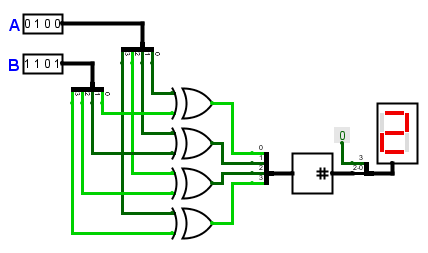
\includegraphics[width=\maxwidth{.95\linewidth}]{gfx/08_20}
	\caption{Hamming Distance}
	\label{fig:08_20}
\end{figure}

The four bits for input \emph{A} and input \emph{B} are wired to four \textsf{XOR} gates then the output of those gates is wired to a \emph{Bit Adder} device. The \textsf{XOR} gates will output a one if the two input bits are different then the bit adder will total how many ones are present at its input. The output of the bit adder is a three-bit number but to make it easier to read that number it is wired to a hex digit display. Since that display needs a four-bit input a constant zero is wired to the most significant bit of the input of the hex digit display.

\subsubsection{Generating Hamming Code}
\label{CL:subsubsec:generating_hamming_code}

Hamming parity is designed so a parity bit is generated for various combinations of bits within a byte in such a way that every data bit is linked to at least three different parity bits. This system can then determine not only that the parity is wrong but which bit is wrong. The cost of a Hamming system is that it adds five parity bits to an eight-bit byte to create a $ 13 $-bit word. Consider the bits for the $ 13 $-bit word in Table \ref{cl:tab:hamming_parity_bits}.

\begin{table}[H]
  \sffamily
  \newcommand{\head}[1]{\textcolor{white}{\textbf{#1}}}		
  \begin{center}
    \rowcolors{2}{gray!10}{white} % Color every other line a light gray
    \begin{tabular}{ccccccccccccc} 
      \rowcolor{black!75}
      \head{$ P_4 $} & \head{$ d_7 $} & \head{$ d_6 $} &
      \head{$ d_5 $} & \head{$ d_4 $} & \head{$ P_3 $} &
      \head{$ d_3 $} & \head{$ d_2 $} & \head{$ d_1 $} &
      \head{$ P_2 $} & \head{$ d_0 $} & \head{$ P_1 $} &
      \head{$ P_0 $} \\
      $ 0 $ & $ 0 $ & $ 0 $ &
      $ 0 $ & $ 0 $ & $ 0 $ &
      $ 0 $ & $ 0 $ & $ 0 $ &
      $ 0 $ & $ 0 $ & $ 0 $ &
      $ 0 $ 
    \end{tabular}
  \end{center}
  \caption{Hamming Parity Bits}
  \label{cl:tab:hamming_parity_bits}
\end{table}

The bits numbered $ P_0 $ to $ P_4 $ are Hamming parity bits and the bits numbered $ d_0 $ to $ d_7 $ are the data bits. The Hamming parity bits are interspersed with the data but they occur in positions zero, one, three, and seven (counting right to left). The following chart shows the data bits that are used to create each parity bit: 

\begin{table}[H]
  \sffamily
  \newcommand{\head}[1]{\textcolor{white}{\textbf{#1}}}		
  \begin{center}
    \rowcolors{2}{gray!10}{white} % Color every other line a light gray
    \begin{tabular}{ccccccccccccc} 
      \rowcolor{black!75}
      \head{$ P_4 $} & \head{$ d_7 $} & \head{$ d_6 $} &
      \head{$ d_5 $} & \head{$ d_4 $} & \head{$ P_3 $} &
      \head{$ d_3 $} & \head{$ d_2 $} & \head{$ d_1 $} &
      \head{$ P_2 $} & \head{$ d_0 $} & \head{$ P_1 $} &
      \head{$ P_0 $} \\
      % Line P0
      \color{gray}{$ 0 $} & \color{gray}{$ 0 $} & $ X $ &
      \color{gray}{$ 0 $} & $ X $ & \color{gray}{$ 0 $} &
      $ X $ & \color{gray}{$ 0 $} & $ X $ &
      \color{gray}{$ 0 $} & $ X $ & \color{gray}{$ 0 $} &
      \color{red}{$ P $} \\
      % Line P1
      \color{gray}{$ 0 $} & \color{gray}{$ 0 $} & $ X $ &
      $ X $ & \color{gray}{$ 0 $} & \color{gray}{$ 0 $} &
      $ X $ & $ X $ & \color{gray}{$ 0 $} &
      \color{gray}{$ 0 $} & $ X $ & \color{red}{$ P $} &
      \color{gray}{$ 0 $} \\
      % Line P2
      \color{gray}{$ 0 $} & $ X $ & \color{gray}{$ 0 $} &
      \color{gray}{$ 0 $} & \color{gray}{$ 0 $} & \color{gray}{$ 0 $} &
      $ X $ & $ X $ & $ X $ &
      \color{red}{$ P $} & \color{gray}{$ 0 $} & \color{gray}{$ 0 $} &
      \color{gray}{$ 0 $} \\
      % Line P3
      \color{gray}{$ 0 $} & $ X $ & $ X $ &
      $ X $ & $ X $ & \color{red}{$ P $} &
      \color{gray}{$ 0 $} & \color{gray}{$ 0 $} & \color{gray}{$ 0 $} &
      \color{gray}{$ 0 $} & \color{gray}{$ 0 $} & \color{gray}{$ 0 $} &
      \color{gray}{$ 0 $} \\
      % Line P4
      \color{red}{$ P $} & $ X $ & \color{gray}{$ 0 $} &
      $ X $ & $ X $ & \color{gray}{$ 0 $} &
      \color{gray}{$ 0 $} & $ X $ & $ X $ &
      \color{gray}{$ 0 $} & $ X $ & \color{gray}{$ 0 $} &
      \color{gray}{$ 0 $} 
    \end{tabular}
  \end{center}
  \caption{Hamming Parity Cover Table}
  \label{cl:tab:hamming_parity_cover_table}
\end{table}

From Table \ref{cl:tab:hamming_parity_cover_table}, line one shows the data bits that are used to set parity bit zero ($ P_{0} $). If data bits $ d0 $, $ d1 $, $ d3 $, $ d4 $, and $ d6 $ are all one then $ P_{0} $ would be one (even parity is assumed). The data bits needed to create the Hamming parity bit are marked in all five lines. A note is necessary about parity bit $ P_4 $. In order to detect transmission errors that are two bits large (that is, two bits were flipped), each data bit needs to be covered by three parity bits. Parity bit $ P_4 $ is designed to provide the third parity bit for any data bits that have only two others. For example, look down the column containing data bit $ d_0 $ and notice that it has only two parity bits ($ P_0 $ and $ P_1 $) before $ P_4 $. By adding $ P_4 $ to the circuit that data bit gets a third parity bit.

As an example of a Hamming code, imagine that this byte needed to be transmitted: $ 0110 \; 1001 $. This number could be placed in the data bit positions of the Hamming table. 

\begin{table}[H]
  \sffamily
  \newcommand{\head}[1]{\textcolor{white}{\textbf{#1}}}		
  \begin{center}
    \rowcolors{2}{gray!10}{white} % Color every other line a light gray
    \begin{tabular}{ccccccccccccc} 
      \rowcolor{black!75}
      \head{$ P_4 $} & \head{$ d_7 $} & \head{$ d_6 $} &
      \head{$ d_5 $} & \head{$ d_4 $} & \head{$ P_3 $} &
      \head{$ d_3 $} & \head{$ d_2 $} & \head{$ d_1 $} &
      \head{$ P_2 $} & \head{$ d_0 $} & \head{$ P_1 $} &
      \head{$ P_0 $} \\
      \color{gray}{$ 0 $} & $ 0 $ & $ 1 $ &
      $ 1 $ & $ 0 $ & \color{gray}{$ 0 $} &
      $ 1 $ & $ 0 $ & $ 0 $ &
      \color{gray}{$ 0 $} & $ 1 $ & \color{gray}{$ 0 $} &
      \color{gray}{$ 0 $}
    \end{tabular}
  \end{center}
  \caption{Hamming Example - Iteration 1}
  \label{cl:tab:hamming_example_iteration_1}
\end{table}

Bit zero, $ P0 $, is designed to generate even parity for data bits $ d_0 $, $ d_1 $, $ d_3 $, $ d_4 $, and $ d_6 $. Since there are three ones in that group, then $ P_0 $ must be one. That has been filled in below (for convenience, the Hamming parity bit pattern for $ P_0 $ is included in the last row of the table). 

\begin{table}[H]
  \sffamily
  \newcommand{\head}[1]{\textcolor{white}{\textbf{#1}}}		
  \begin{center}
    \rowcolors{2}{gray!10}{white} % Color every other line a light gray
    \begin{tabular}{ccccccccccccc} 
      \rowcolor{black!75}
      \head{$ P_4 $} & \head{$ d_7 $} & \head{$ d_6 $} &
      \head{$ d_5 $} & \head{$ d_4 $} & \head{$ P_3 $} &
      \head{$ d_3 $} & \head{$ d_2 $} & \head{$ d_1 $} &
      \head{$ P_2 $} & \head{$ d_0 $} & \head{$ P_1 $} &
      \head{$ P_0 $} \\
      \color{gray}{$ 0 $} & $ 0 $ & $ 1 $ &
      $ 1 $ & $ 0 $ & \color{gray}{$ 0 $} &
      $ 1 $ & $ 0 $ & $ 0 $ &
      \color{gray}{$ 0 $} & $ 1 $ & \color{gray}{$ 0 $} &
      \color{red}{$ 1 $} \\
      % Line P0
      \color{gray}{$ 0 $} & \color{gray}{$ 0 $} & $ X $ &
      \color{gray}{$ 0 $} & $ X $ & \color{gray}{$ 0 $} &
      $ X $ & \color{gray}{$ 0 $} & $ X $ &
      \color{gray}{$ 0 $} & $ X $ & \color{gray}{$ 0 $} &
      \color{red}{$ P $} \\      
    \end{tabular}
  \end{center}
  \caption{Hamming Example - Iteration 2}
  \label{cl:tab:hamming_example_iteration_2}
\end{table}

Bit one, $ P_1 $, is designed to generate even parity for data bits $ d_0 $, $ d_2 $, $ d_3 $, $ d_5 $, and $ d_6 $. Since there are four ones in that group, then $ P_1 $ must be zero. That has been filled in below. 

\begin{table}[H]
  \sffamily
  \newcommand{\head}[1]{\textcolor{white}{\textbf{#1}}}		
  \begin{center}
    \rowcolors{2}{gray!10}{white} % Color every other line a light gray
    \begin{tabular}{ccccccccccccc} 
      \rowcolor{black!75}
      \head{$ P_4 $} & \head{$ d_7 $} & \head{$ d_6 $} &
      \head{$ d_5 $} & \head{$ d_4 $} & \head{$ P_3 $} &
      \head{$ d_3 $} & \head{$ d_2 $} & \head{$ d_1 $} &
      \head{$ P_2 $} & \head{$ d_0 $} & \head{$ P_1 $} &
      \head{$ P_0 $} \\
      \color{gray}{$ 0 $} & $ 0 $ & $ 1 $ &
      $ 1 $ & $ 0 $ & \color{gray}{$ 0 $} &
      $ 1 $ & $ 0 $ & $ 0 $ &
      \color{gray}{$ 0 $} & $ 1 $ & \color{red}{$ 0 $} &
      $ 1 $ \\
      % Line P1
      \color{gray}{$ 0 $} & \color{gray}{$ 0 $} & $ X $ &
      $ X $ & \color{gray}{$ 0 $} & \color{gray}{$ 0 $} &
      $ X $ & $ X $ & \color{gray}{$ 0 $} &
      \color{gray}{$ 0 $} & $ X $ & \color{red}{$ P $} &
      \color{gray}{$ 0 $} \\
    \end{tabular}
  \end{center}
  \caption{Hamming Example - Iteration 3}
  \label{cl:tab:hamming_example_iteration_3}
\end{table}

Bit three, $ P_2 $, is designed to generate even parity for data bits $ d_1 $, $ d_2 $, $ d_3 $, and $ d_7 $. Since there is one one in that group, then $ P_2 $ must be one. That has been filled in below. 

\begin{table}[H]
  \sffamily
  \newcommand{\head}[1]{\textcolor{white}{\textbf{#1}}}		
  \begin{center}
    \rowcolors{2}{gray!10}{white} % Color every other line a light gray
    \begin{tabular}{ccccccccccccc} 
      \rowcolor{black!75}
      \head{$ P_4 $} & \head{$ d_7 $} & \head{$ d_6 $} &
      \head{$ d_5 $} & \head{$ d_4 $} & \head{$ P_3 $} &
      \head{$ d_3 $} & \head{$ d_2 $} & \head{$ d_1 $} &
      \head{$ P_2 $} & \head{$ d_0 $} & \head{$ P_1 $} &
      \head{$ P_0 $} \\
      \color{gray}{$ 0 $} & $ 0 $ & $ 1 $ &
      $ 1 $ & $ 0 $ & \color{gray}{$ 0 $} &
      $ 1 $ & $ 0 $ & $ 0 $ &
      \color{red}{$ 1 $} & $ 1 $ & $ 0 $ &
      $ 1 $ \\
      % Line P2
      \color{gray}{$ 0 $} & $ X $ & \color{gray}{$ 0 $} &
      \color{gray}{$ 0 $} & \color{gray}{$ 0 $} & \color{gray}{$ 0 $} &
      $ X $ & $ X $ & $ X $ &
      \color{red}{$ P $} & \color{gray}{$ 0 $} & \color{gray}{$ 0 $} &
      \color{gray}{$ 0 $} \\
    \end{tabular}
  \end{center}
  \caption{Hamming Example - Iteration 4}
  \label{cl:tab:hamming_example_iteration_4}
\end{table}

Bit seven, $ P_3 $, is designed to generate even parity for data bits $ d_4 $, $ d_5 $, $ d_6 $, and $ d_7 $. Since there are two ones in that group, then $ P_3 $ must be zero. That has been filled in below. 

\begin{table}[H]
  \sffamily
  \newcommand{\head}[1]{\textcolor{white}{\textbf{#1}}}		
  \begin{center}
    \rowcolors{2}{gray!10}{white} % Color every other line a light gray
    \begin{tabular}{ccccccccccccc} 
      \rowcolor{black!75}
      \head{$ P_4 $} & \head{$ d_7 $} & \head{$ d_6 $} &
      \head{$ d_5 $} & \head{$ d_4 $} & \head{$ P_3 $} &
      \head{$ d_3 $} & \head{$ d_2 $} & \head{$ d_1 $} &
      \head{$ P_2 $} & \head{$ d_0 $} & \head{$ P_1 $} &
      \head{$ P_0 $} \\
      \color{gray}{$ 0 $} & $ 0 $ & $ 1 $ &
      $ 1 $ & $ 0 $ & \color{red}{$ 0 $} &
      $ 1 $ & $ 0 $ & $ 0 $ &
      $ 1 $ & $ 1 $ & $ 0 $ &
      $ 1 $ \\
      % Line P3
      \color{gray}{$ 0 $} & $ X $ & $ X $ &
      $ X $ & $ X $ & \color{red}{$ P $} &
      \color{gray}{$ 0 $} & \color{gray}{$ 0 $} & \color{gray}{$ 0 $} &
      \color{gray}{$ 0 $} & \color{gray}{$ 0 $} & \color{gray}{$ 0 $} &
      \color{gray}{$ 0 $} \\
    \end{tabular}
  \end{center}
  \caption{Hamming Example - Iteration 5}
  \label{cl:tab:hamming_example_iteration_5}
\end{table}

Bit eight, $ P_4 $, is designed to generate even parity for data bits $ d_0 $, $ d_1 $, $ d_2 $, $ d_4 $, $ d_5 $, and $ d_7 $. Since there are two ones in that group, then $ P_4 $ must be zero. That has been filled in below. 

\begin{table}[H]
  \sffamily
  \newcommand{\head}[1]{\textcolor{white}{\textbf{#1}}}		
  \begin{center}
    \rowcolors{2}{gray!10}{white} % Color every other line a light gray
    \begin{tabular}{ccccccccccccc} 
      \rowcolor{black!75}
      \head{$ P_4 $} & \head{$ d_7 $} & \head{$ d_6 $} &
      \head{$ d_5 $} & \head{$ d_4 $} & \head{$ P_3 $} &
      \head{$ d_3 $} & \head{$ d_2 $} & \head{$ d_1 $} &
      \head{$ P_2 $} & \head{$ d_0 $} & \head{$ P_1 $} &
      \head{$ P_0 $} \\
      \color{red}{$ 0 $} & $ 0 $ & $ 1 $ &
      $ 1 $ & $ 0 $ & $ 0 $ &
      $ 1 $ & $ 0 $ & $ 0 $ &
      $ 1 $ & $ 1 $ & $ 0 $ &
      $ 1 $ \\
      % Line P4
      \color{red}{$ P $} & $ X $ & \color{gray}{$ 0 $} &
      $ X $ & $ X $ & \color{gray}{$ 0 $} &
      \color{gray}{$ 0 $} & $ X $ & $ X $ &
      \color{gray}{$ 0 $} & $ X $ & \color{gray}{$ 0 $} &
      \color{gray}{$ 0 $} 
    \end{tabular}
  \end{center}
  \caption{Hamming Example - Iteration 6}
  \label{cl:tab:hamming_example_iteration_6}
\end{table}

When including Hamming parity, the byte $ 0110 \; 1001 $ is converted to: $ 0 \; 0110 \; 0100 \; 1101 $.

In Figure \ref{fig:08_21}, a 11-bit input, \emph{A}, is used to create a 16-bit word that includes Hamming parity bits. In the illustration, input $ 010 \; 0111 \; 0111 $ is converted to $ 1010 \; 0100 \; 1110 \; 1111 $.  

\begin{figure}[H]
	\centering
	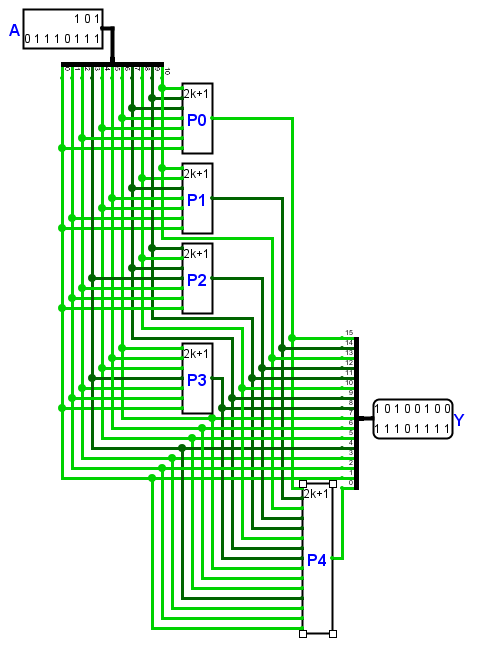
\includegraphics[width=\maxwidth{.95\linewidth}]{gfx/08_21}
	\caption{Generating Hamming Parity}
	\label{fig:08_21}
\end{figure}

The process used by the circuit in Figure \ref{fig:08_21} is to wire each of the input bits to various parity generators and then combine the outputs of those parity generators, along with the original bits, into a single 16-bit word. While the circuit has a lot of wired connections the concept is fairly simple. \textsf{P0} calculates the parity for input bits $ 0, 1, 3, 4, 6, 8, 10 $. That is then wired to the least significant bit of output \emph{Y}.

\subsubsection{Checking Hamming Code}
\label{CL:subsubsec:checking_hamming_code}

To check the accuracy of the data bits in a word that contains Hamming parity bits the following general process is used:

\begin{enumerate}
  \item Calculate the Hamming Parity Bit for each of the bit groups exactly like when the parity was first calculated.
  \item Compare the calculated Hamming Parity bits with the parity bits found in the original binary word.
  \item If the parity bits match then there is no error. If the parity bits do not match then the bad bit can be corrected by using the pattern of parity bits that do not match.
\end{enumerate}

As an example, imagine that bit eight (last bit in the first group of four) in the Hamming code created above was changed from zero to one: $ 0 \; 011\underline{1} \; 0100 \; 1101 $ (this is bit $ d_4 $).  Table \ref{cl:tab:hamming_parity_cover_table_reproduced} shows that Hamming Bits $ P_0 $, $ P_3 $, and $ P_4 $ would now be incorrect since $ d_4 $ is used to create those parity bits.

\begin{table}[H]
  \sffamily
  \newcommand{\head}[1]{\textcolor{white}{\textbf{#1}}}		
  \begin{center}
    \rowcolors{2}{gray!10}{white} % Color every other line a light gray
    \begin{tabular}{ccccccccccccc} 
      \rowcolor{black!75}
      \head{$ P_4 $} & \head{$ d_7 $} & \head{$ d_6 $} &
      \head{$ d_5 $} & \head{$ d_4 $} & \head{$ P_3 $} &
      \head{$ d_3 $} & \head{$ d_2 $} & \head{$ d_1 $} &
      \head{$ P_2 $} & \head{$ d_0 $} & \head{$ P_1 $} &
      \head{$ P_0 $} \\
      % Line P0
      \color{gray}{$ 0 $} & \color{gray}{$ 0 $} & $ X $ &
      \color{gray}{$ 0 $} & \cellcolor{yellow!70!white}$ X $ & \color{gray}{$ 0 $} &
      $ X $ & \color{gray}{$ 0 $} & $ X $ &
      \color{gray}{$ 0 $} & $ X $ & \color{gray}{$ 0 $} &
      \color{red}{$ P $} \\
      % Line P1
      \color{gray}{$ 0 $} & \color{gray}{$ 0 $} & $ X $ &
      $ X $ & \color{gray}{$ 0 $} & \color{gray}{$ 0 $} &
      $ X $ & $ X $ & \color{gray}{$ 0 $} &
      \color{gray}{$ 0 $} & $ X $ & \color{red}{$ P $} &
      \color{gray}{$ 0 $} \\
      % Line P2
      \color{gray}{$ 0 $} & $ X $ & \color{gray}{$ 0 $} &
      \color{gray}{$ 0 $} & \color{gray}{$ 0 $} & \color{gray}{$ 0 $} &
      $ X $ & $ X $ & $ X $ &
      \color{red}{$ P $} & \color{gray}{$ 0 $} & \color{gray}{$ 0 $} &
      \color{gray}{$ 0 $} \\
      % Line P3
      \color{gray}{$ 0 $} & $ X $ & $ X $ &
      $ X $ & \cellcolor{yellow!70!white}$ X $ & \color{red}{$ P $} &
      \color{gray}{$ 0 $} & \color{gray}{$ 0 $} & \color{gray}{$ 0 $} &
      \color{gray}{$ 0 $} & \color{gray}{$ 0 $} & \color{gray}{$ 0 $} &
      \color{gray}{$ 0 $} \\
      % Line P4
      \color{red}{$ P $} & $ X $ & \color{gray}{$ 0 $} &
      $ X $ & \cellcolor{yellow!70!white}$ X $ & \color{gray}{$ 0 $} &
      \color{gray}{$ 0 $} & $ X $ & $ X $ &
      \color{gray}{$ 0 $} & $ X $ & \color{gray}{$ 0 $} &
      \color{gray}{$ 0 $} 
    \end{tabular}
  \end{center}
  \caption{Hamming Parity Cover Table Reproduced}
  \label{cl:tab:hamming_parity_cover_table_reproduced}
\end{table}

Since the only data bit that uses these three parity bits is $ d_4 $ then that one bit can be inverted to correct the data in the eight-bit byte.

The circuit illusted in Figure \ref{fig:08_22} realizes a Hamming parity check. Notice that the input is the same 16-bit word generated in the circuit in Figure \ref{fig:08_21} except bit eight (the last bit on the top row of the input) has been complemented. The circuit reports that bit eight is in err so it would not only alert an operator that something is wrong with this data but it would also be able to automatically correct the wrong bit.

\begin{figure}[H]
	\centering
	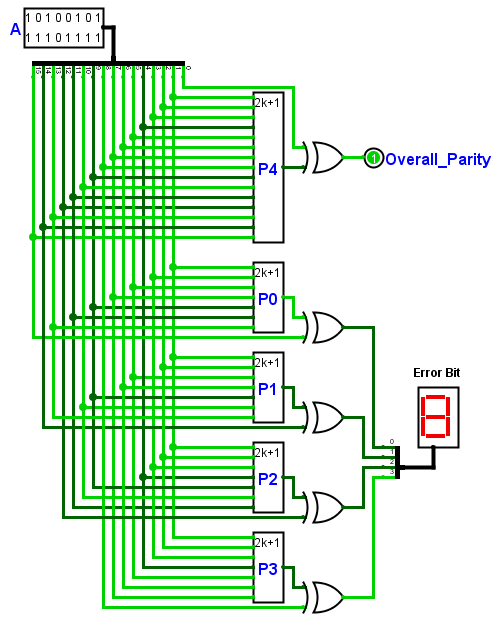
\includegraphics[width=\maxwidth{.95\linewidth}]{gfx/08_22}
	\caption{Checking Hamming Parity}
	\label{fig:08_22}
\end{figure}


\subsection{Hamming Code Notes}
\label{CL:subsec:hamming_code_notes}

\begin{itemize}
  \item When a binary word that includes Hamming parity is checked to verify the accuracy of the data bits using three overlapping parity bits, as developed in this book, one-bit errors can be corrected and two-bit errors can be detected. This type of system is often called \gls{secded} and is commonly used in computer memories to ensure data integrity.

  \item While it seems wasteful to add five Hamming bits to an eight-bit byte (a 62.5\% increase in length), the number of bits needed for longer words does not continue to increase at that rate. Hamming bits are added to a binary word in multiples of powers of two. For example, to cover a 32-bit word only seven Hamming bits are needed, an increase of only about 22.\%; and to cover a 256-bit word only $ 10 $ Hamming bits are needed, an increase of just under 4\%.

  \item This lesson counts bits from right-to-left and considers the first position as bit zero, which matches with the bit counting pattern used throughout the book. However, many authors and online resources count Hamming bits from left-to-right and consider the left-most position as bit one because that is a natural way to count.
\end{itemize}

\subsection{Sample Problems}
\label{CL:subsec:sample_problems_error_detection}

The following problems are provided for practice. 

\begin{table}[H]
  \sffamily
  \newcommand{\head}[1]{\textcolor{white}{\textbf{#1}}}    
  \begin{center}
    \rowcolors{2}{gray!10}{white} % Color every other line a light gray
    \begin{tabular}{cc} 
      \rowcolor{black!75}
      \head{8-Bit Byte} & \head{With Hamming} \\
      $ 11001010 $ & $ 1110011011001 $ \\
      $ 10001111 $ & $ 1100001110111 $ \\
      $ 01101101 $ & $ 0011011100111 $ \\
      $ 11100010 $ & $ 0111000010000 $ \\
      $ 10011011 $ & $ 1100111011100 $ \\
    \end{tabular}
  \end{center}
  \caption{Hamming Parity Examples}
  \label{CL:tab:hamming_parity_examples}
\end{table}

\begin{table}[H]
  \sffamily
  \newcommand{\head}[1]{\textcolor{white}{\textbf{#1}}}    
  \begin{center}
    \rowcolors{2}{gray!10}{white} % Color every other line a light gray
    \begin{tabular}{cc} 
      \rowcolor{black!75}
      \head{Hamming With Error} & \head{Error Bit} \\
      $ 0110101011001 $ & 1 \\
      $ 1100000100110 $ & 3 \\
      $ 0000100001100 $ & 5 \\
      $ 1110111011010 $ & 9 \\
      $ 1110010100110 $ & 12 \\
    \end{tabular}
  \end{center}
  \caption{Hamming Parity Errors}
  \label{CL:tab:hamming_parity_errors}
\end{table}
